\begin{filecontents}{preliminary.sty}
\ProvidesPackage{preliminary}
%\DeclareOption{draft}{%
  \AtBeginDocument{%
    \renewcommand\maketitlehookc
\ProcessOptions
\RequirePackage{titling}
\endinput
\end{filecontents}

\documentclass[12pt, a4paper]{article}
\usepackage{setspace}
\usepackage{ragged2e}
\usepackage[centertags,reqno]{amsmath}
\usepackage{amssymb}
\usepackage{graphics,subfigure}
\usepackage[dvips]{graphicx}
\usepackage[dvipsnames]{xcolor}
\usepackage[hidelinks]{hyperref}
\usepackage{appendix}
\usepackage{natbib}
\usepackage{verbatim,color}
\usepackage{pdflscape}
\usepackage[showframe=false]{geometry}
\usepackage{changepage}
\usepackage{xcolor}
\usepackage{eurosym}
\usepackage{textcomp}
\usepackage[open,openlevel=1]{bookmark}
\usepackage{multirow}
\usepackage{caption}
\usepackage{hyphenat}
\newcommand{\mybox}[2]{{\color{#1}\fbox{\normalcolor#2}}}
\doublespacing

% Exception to hyphenation
\hyphenation{par-ti-ci-pants}
\hyphenation{par-ti-ci-pant}
\hyphenation{Hy-po-the-sis}
\hyphenation{ex-pe-ri-ment}
\hyphenation{ex-pe-ri-ments}

% Allows bigger tables to be scaled down
\usepackage{adjustbox}

%From my paper with Raymond
\usepackage{tabularx,calc}
\usepackage{dcolumn}                    % Aligns tables on the decimal point
\newcolumntype{d}[1]{D{.}{.}{#1}}       %       Aligns on dot
\newcolumntype{.}{D{.}{.}{3.5}}         %       Somehow it works better
\newcolumntype{C}{@{\extracolsep{.6cm}}c@{\extracolsep{0pt}}}
\usepackage{threeparttable}
\usepackage{siunitx,booktabs}
\sisetup{
    detect-all,
    round-integer-to-decimal = true,
    group-digits             = true,
    group-minimum-digits     = 4,
    group-separator          = {\,},
    table-align-text-pre     = false,
    table-align-text-post    = false,
    input-signs              = + -,
    input-symbols            = {*} {**} {***},
    input-open-uncertainty   = ,
    input-close-uncertainty  = ,
    retain-explicit-plus
}

% Commands to name appendices Appendix A, Appendix B, etc.
\makeatletter
%% The "\@seccntformat" command is an auxiliary command
%% (see pp. 26f. of 'The LaTeX Companion,' 2nd. ed.)
\def\@seccntformat#1{\@ifundefined{#1@cntformat}%
   {\csname the#1\endcsname\quad}  % default
   {\csname #1@cntformat\endcsname}% enable individual control
}
\let\oldappendix\appendix %% save current definition of \appendix
\renewcommand\appendix{%
    \oldappendix
    \newcommand{\section@cntformat}{\appendixname~\thesection\quad}
}

%Adds text specifying it is a preliminary version
\usepackage{preliminary}

\title{Eliciting Minimum Acceptable Probabilities \\
\Large Pre-Analysis Plan}
\author{Martin Strobel  \and Maria Polipciuc\thanks{Maastricht University. Email: \url{m.polipciuc@maastrichtuniversity.nl}. We thank Elias Tsakas for valuable comments.}}
\date{\today	\vspace{1cm}}
\titlepage


\begin{document}
\begin{titlepage}
\clearpage\maketitle
\thispagestyle{empty}

\end{titlepage}
\section{Main page description (public)}
\large \textcolor{RoyalBlue}{\textbf{Interventions}}

\normalsize \noindent \textcolor{NavyBlue}{\textbf{Intervention(s)}}

We compare minimum acceptable probabilities (MAPs) for which a participant considers a binary lottery equally desirable to a sure payoff across treatments within individual.
Individuals have to decide in randomized order in three scenarios (treatments).
The treatments vary the distribution of the winning probability of the lottery.

\noindent \textcolor{NavyBlue}{\textbf{Trial Start Date}}
\textcolor{red}{Will we have a trial, for instance to test understanding of instructions?}

\noindent \textcolor{NavyBlue}{\textbf{Intervention Start Date}}

TBD

\noindent \textcolor{NavyBlue}{\textbf{Intervention End Date}}

TBD



\large \noindent \textcolor{RoyalBlue}{\textbf{Primary Outcomes}}

\normalsize \noindent \textcolor{NavyBlue}{\textbf{Primary Outcomes (end points)}}

MAPs

\noindent \textcolor{NavyBlue}{\textbf{Primary Outcomes (explanation)}}

The MAPs are elicited as indifference values. 



\large \noindent \textcolor{RoyalBlue}{\textbf{Experimental Design}}

\normalsize \noindent \textcolor{NavyBlue}{\textbf{Experimental Design}}

We elicit MAPs in an online experiment in a lottery similar to the \textit{Decision Problem} in \cite{Bohnet2004}.
The aim is to test an assumption required for the MAP elicitation procedure to be incentive-compatible.
Specifically, we test whether there is evidence that participants' declared MAPs are independent of the underlying distribution from which the probability of success of the gamble is drawn.
We do this by exogenously manipulating this distribution, and comparing the resulting MAPs across treatments.

\noindent \textcolor{NavyBlue}{\textbf{Experimental Design Details}}

Not available

\noindent \textcolor{NavyBlue}{\textbf{Randomization Method}}

Computer

\noindent \textcolor{NavyBlue}{\textbf{Randomization Unit}}

Individual

\noindent \textcolor{NavyBlue}{\textbf{Was the treatment clustered?}}

No

\noindent \textcolor{NavyBlue}{\textbf{Planned Number of Observations}}

TBD
    
\noindent \textcolor{NavyBlue}{\textbf{Was IRB approval obtained (only for ``In Development" and ``On-going" trials)?}} If so, also

        IRB Name
        
        IRB Approval Date
        
        IRB Approval Number





\section{Introduction}
The Minimum Acceptable Probability (MAP) is an elicitation procedure for an indifference value (expressed as the probability or as the number of favorable outcomes) between a sure payoff and trusting someone.
In other words, it is the value which makes an individual indifferent between engaging and not engaging in a trusting interaction.

The concept was introduced by \cite{Bohnet2004} and it has been used—with slight variations—to elicit a determinant of trust, betrayal aversion, in a difference-in-difference design.
This procedure is incentive compatible if ``a principal adheres to the Substitution Axiom of von Neumann-Morgenstern utility [...] A MAP is a cutoff value relating to preferences, and the estimated value of $p^*$ [\textit{NR: the winning probability}] should not affect it.'' \citep[p. 298]{Bohnet2008}.
While empirical violations of this axiom---which implies expected utility---have been documented \cite[see footnote 5 on p. 275 in][for a list of studies finding empirical violations]{Li2020a}, to our knowledge it is not yet established whether this violation is empirically relevant in the context of the MAP elicitation procedure.\footnote{
\textcolor{red}{Another important point is the following observation made in footnote 4 on p. 815 in \cite{Bohnet2010}: ``Note that a principal cannot affect the probability he or she receives in the lottery, because it in no way relates to the answer that he or she provides.''}
\textcolor{red}{This is true by design; however, we believe that there is another dimension of risk exposure than the probability received in the lottery that the participant can control through their MAP.}
\textcolor{red}{The participant can be viewed as facing a compound risk, which consists of (i) the probability received in the lottery and (ii) the probability that they receive a lottery with a certain winning probability or higher at a certain MAP, which is determined by its cumulative density (or mass, if the distribution is discrete) function.}
\textcolor{red}{From this, the underlying distribution of the winning probability in the lottery may influence the MAP due to its impact on (ii).}
\textcolor{red}{An implication is that the difference between treatments might be due to different underlying distributions of the winning probability across treatments, not to the different nature of the lotteries (risky/social/strategic).}
\textcolor{red}{In other words, the difference might be due to risk aversion---this could potentially explain why several studies which keep subjective probabilities constant across treatments and do not find evidence of betrayal aversion \citep{Fetchenhauer2012,Polipciuc2020}.}
}


This paper investigates whether the MAP is influenced by a participant’s subjective expectation of the chance of a favorable outcome. 
Specifically, we remove the social and strategic aspects of a trust decision, and study the MAP for accepting a risky lottery.
We manipulate participants’ subjective expectations about the lottery’s winning chances by varying the ``world’’ in which they report a MAP.
The experiment consists of three ``worlds'' (treatments), which participants experience sequentially in randomized order.
For each decision, the world is described to participants before the MAP elicitation, and it is characterized by a distribution over winning probabilities.
A state of the world is a probability drawn from this distribution prior to decision-making, but about which the participant is only informed after having made his/her decision.
Should participants change their MAP depending on the world they face, this is evidence that the MAP elicitation procedure (which uses the strategy method) is not incentive compatible unless one accounts for subjective expectations.\footnote{
When uncertainty is resolved—even if this is irrelevant for strategic or informational purposes—has also been shown to matter for decisions \citep[see footnote 11 on p. 29 in][]{Johnson2019}.
The experiment jointly tests whether different ``worlds'' matter, in a context where uncertainty is resolved after making the decision (the actual state of the world is revealed to participants after they state their MAP).

In BZ, the state of the world is determined before participants make a decision (but they are not told from which ``world'' i.e. distribution of states it has been drawn).
Similarly to our experiment, they are only informed about the state of the world after having made their decision.
}

Below we present the sample selection procedure, the experimental design, and the empirical strategy.



\section{Research Strategy}
This project will collect experimental data on an online platform dedicated to academic research, Prolific, in February 2021. Participants will be exposed randomly to one of six sequences of worlds.
There are three possible worlds: one in which the winning probability is uniformly distributed, one in which its distribution has a right skew, and one in which its distribution has a left skew.
In each world, they have to decide in \citeauthor{Bohnet2004}'s (\citeyear{Bohnet2004}) \textit{Decision Problem} (p. 469). Given the complexity of the tasks, we will recruit participants with completed higher education \textcolor{red}{(also students?)}, to increase the chances that task comprehension is not an issue.

The pre-analysis plan will be registered at the AEA RCT registry before the start of the data collection.

\subsection{Recruitment}
Participants are registered users on the online platform Prolific.
This platform is tailored for academic research, and gathers demographics about registered users.
We will send an invitation to the experiment only to participants who have completed higher education \textcolor{red}{(maybe also to students?)}, for the reasons mentioned above. 



\section{Design}
The study will consist of three parts.
The first part will be an attention and understanding check (unincentivized).
Only those passing this check will be directed to the main part, which is incentivized.
After this, those who have completed the second part will go through a survey.

As mentioned above, participants in the experiment will be asked to state their MAP in a \textit{Decision Problem}: what is their MAP for taking a gamble rather than accepting a sure payoff?
The experiment will combine a within-subject design (with all participants going through all treatments sequentially) with a between-subject design.

Below we present the design and instructions in more detail.

\subsection{Attention and understanding check}
Here will follow the exact wording of the questions.

\subsection{MAP elicitation}
Here will follow the exact wording of each ``world'' description.

WORLD 1

WORLD 2

WORLD 3

\textcolor{red}{For how to phrase the MAP question, my suggestion is to take inspiration from} \cite{Johnson2019} \textcolor{red}{(forthcoming in the Journal of Decision and Uncertainty), as per their example on page E.2 in their online appendix here:} \url{https://personal.eur.nl/wakker/oldpsabs.htm#prince21.1} (this is a WTA task, so it has to be adapted).
I also post it here:

\begin{figure}[h!]
  \centering
 {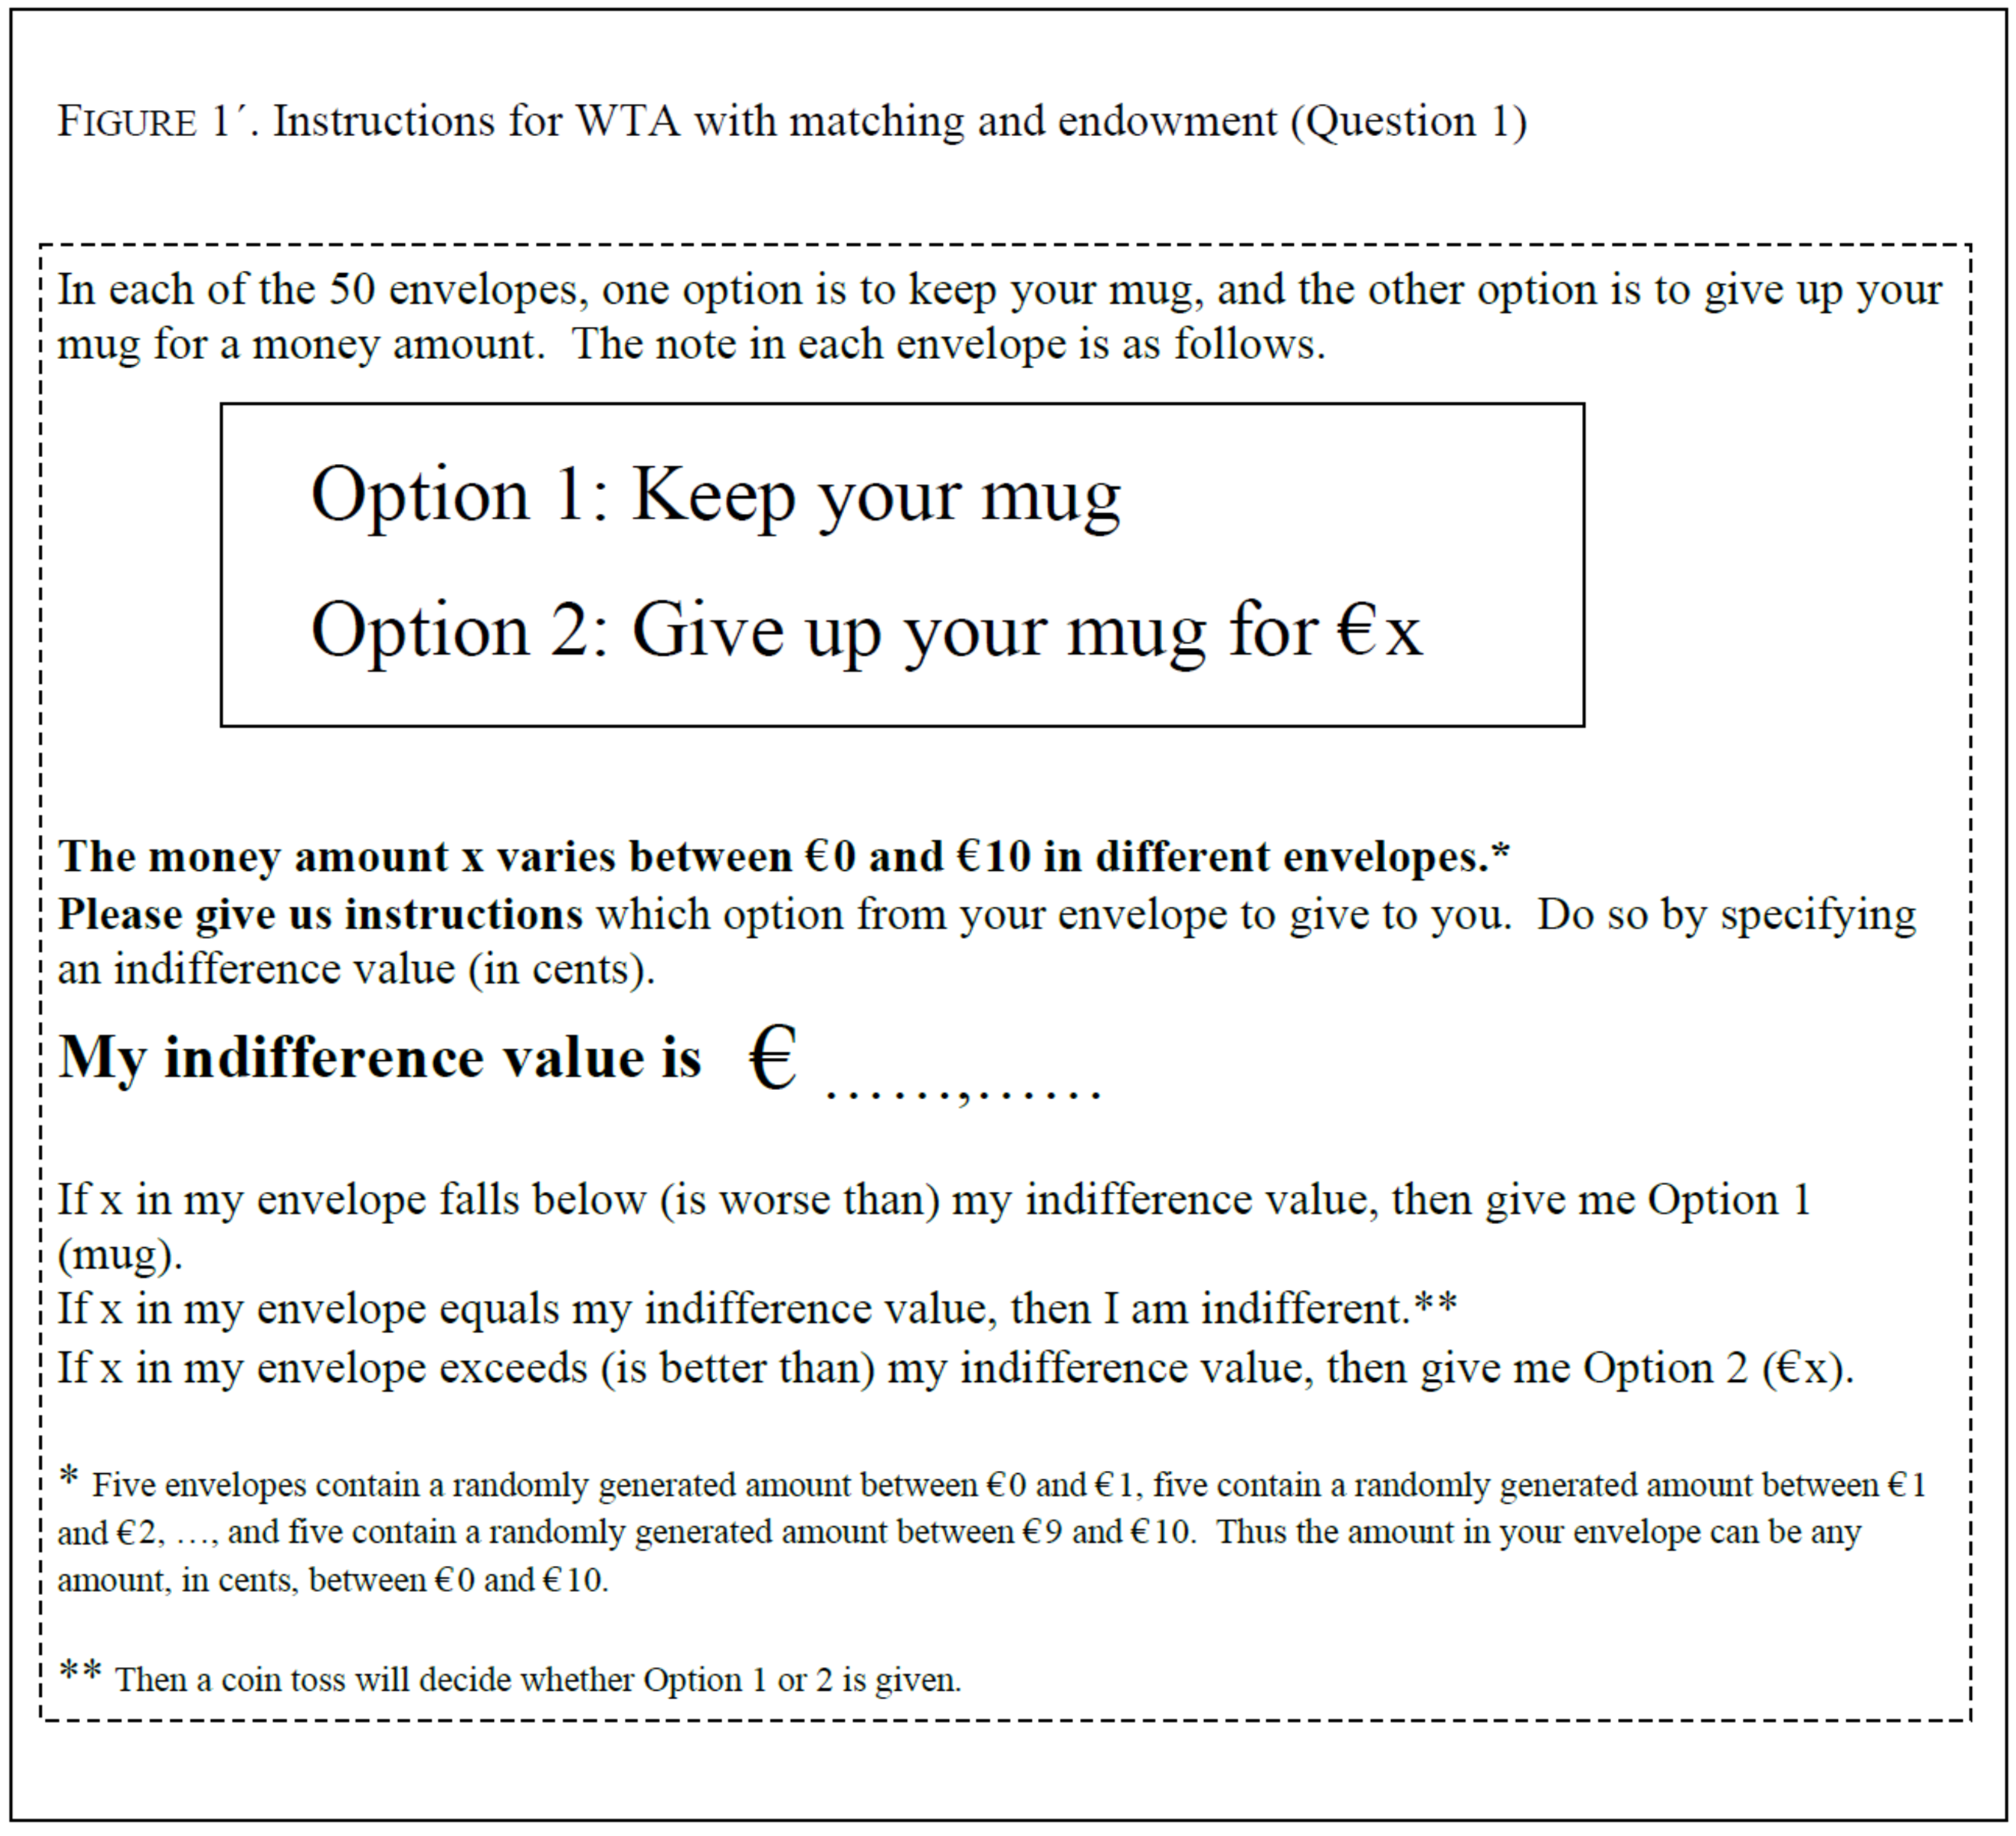
\includegraphics[width=0.95\linewidth]{Wakker_image.pdf}}
  \label{fig:instr}
\end{figure}

\subsection{Survey}
Here will follow the exact wording of the questions.



\section{Empirical Strategy}
The experiment is meant to study whether the world in which one chooses the indifference value for the MAP influences the MAP.
If \cite{Bohnet2008} are right and the estimated value of the true winning probability does not influence MAP, then we should not see significant differences between treatments.

However, there is evidence that individuals change their views on what is a fair payoff/what they can request as an indifference value depending on the world they are in \citep{Bohnet2008,Bohnet2010}.\footnote{
\cite{Bohnet2010} discuss culturally different reference points for trustworthiness which can influence the MAP.
The claim we test is different: that (some of) the observed difference between treatments in their paper and many others is not due to the social or strategic dimensions of a trusting interaction, but to a difference in underlying distributions of the probability of winning---which could influence the MAP through changing reference points for what is a fair deal.
}

A world $A$ is friendlier than another world $B$ if the cumulative density (mass) function of $p^*$ in $A$ is below the cumulative density (mass) function of $p^*$ in $B$ for $p^*$ in [0,1], where the range of states for worlds $A$ and $B$ is the same.
We expect this threshold to be higher in ``friendlier'' worlds, and lower in ``less friendly'' worlds, for instance because of (i) a different perception of what is a fair chance or (ii) anchoring on higher values (for instance, a higher mean of $p^*$) or (iii) a different thrill from gambling or (iv) different aspiration levels or (v) different reference points---leading to different loss aversion effects or (vi) higher order risk attitudes or \textcolor{red}{think of other reasons}.\footnote{
The post-experimental survey could shed some light on whether \textcolor{red}{(some of)} the factors matter.
We leave it to future research to study the mechanisms at play, should we find that results in line with our expectations.
}

This leads to the following hypotheses.

\subsection{Hypotheses}
\subsubsection{Main hypotheses}
\noindent \textbf{Hypothesis 1} \quad \textit{The MAP in the world with left skew (more mass on high values of $p^*$) is higher than the MAP in the world with right skew (more mass on low values of $p^*$).}

\noindent \textbf{Hypothesis 2} \quad \textit{The MAP in the world with left skew (more mass on high values of $p^*$) is higher than the MAP in the world with a uniform distribution over $p^*$.}

\noindent \textbf{Hypothesis 3} \quad \textit{The MAP in the world with right skew (more mass on low values of $p^*$) is lower than the MAP in the world with a uniform distribution over $p^*$.}

\subsubsection{Heterogeneity}
Since the MAP is a way to gauge risk aversion, we expect that in the same world, females state higher MAPs than males on average.

\noindent \textbf{Hypothesis 4} \quad \textit{Within each world, females require higher MAPs on average than males.}

Our treatments vary the objective distribution of the winning probability.
How subjects process these probabilities might depend on things like (i) their optimism/pessimism \textcolor{red}{etc}.
These heterogeneity analyses will be based on subsamples resulting from answers to the post-experimental survey.\footnote{
Gender is among the demographics which we can obtain from Prolific.
}

\noindent \textbf{Hypothesis 5} \quad \textit{Within each world, more optimistic individuals require lower MAPs on average than pessimistic individuals.}

\textcolor{red}{Maybe a question on taking risks? Concerns with fairness? External reference point for earnings e.g. how much should a 45-minute survey pay for you to be willing to take it (if it pays a fixed amount)?--> if international sample, allow them to select currency}



\subsection{Specifications and Analysis}
We present the OLS regressions which will be used to test the hypotheses.
Additionally, we will also run non-parametric Mann-Whitney U tests.

The main hypotheses (1--3) will be tested using the following regression:
\begin{equation} \label{eq:1}
MAP_i = \beta + \beta_L L + \beta_R R + \epsilon_i
\end{equation}

\noindent where $MAP_i$ is the MAP chosen by participant $i$, $L$ is an indicator which takes the value of 1 if the decision was made in the left skew world, $R$ is an indicator which is 1 if the decision was made in the right skew world and $\epsilon_i$ is a random error term.
Standard errors in the estimation will be clustered at the individual level.

For heterogeneity analyses, we will interact all terms in equation (\ref{eq:1}) with an indicator variable corresponding to each specific hypothesis.
For instance, for Hypothesis 5, all terms will be interacted with indicator variable $F_i$, which takes the value 1 if the participant is female:
\begin{equation} \label{eq:2}
MAP_i = \beta + \beta^F F_i + \beta_L L + \beta_L^F L F_i + \beta_R R + \beta_R^F R F_i + \epsilon_i
\end{equation}

The formal statements of the hypotheses are in the Appendix.

\clearpage
\pagebreak
\bibliographystyle{apalike}
\bibliography{Communities}

\clearpage
\pagebreak

\appendix
\section{Hypothesis Testing}
\label{section:appendixa}
\setcounter{figure}{0}
\setcounter{table}{0}
\renewcommand{\thefigure}{A.\arabic{figure}}
\renewcommand{\thetable}{A.\arabic{table}}

\subsection{Hypothesis 1}
$H0: \beta_L - \beta_R = 0 \\
H1: \beta_L - \beta_R > 0$

\subsection{Hypothesis 2}
$H0: \beta_L = 0 \\
H1: \beta_L > 0$

\subsection{Hypothesis 3}
$H0: \beta_R = 0 \\
H1: \beta_R > 0$

\subsection{Hypothesis 4}
Within each world:

\noindent $H0: \beta^F = 0 \\
H1: \beta^F > 0$

\noindent or

\noindent $H0: \beta^F + \beta_L^F = 0 \\
H1: \beta^F + \beta_L^F > 0$

\noindent or

\noindent $H0: \beta^F + \beta_R^F = 0 \\
H1: \beta^F + \beta_R^F > 0$

\subsection{Hypothesis 5}
Analogous to Hypothesis 4.

\end{document}